\documentclass[11pt]{article}
\usepackage[table]{xcolor}
\usepackage{amsmath} 
\usepackage{hyperref}
\usepackage{graphicx}
\usepackage{subcaption}
\usepackage{sectsty}
\usepackage{amssymb}
 \usepackage{lipsum}
\usepackage{titlesec}
\usepackage{romannum}
\usepackage{enumitem}
\usepackage{mathtools}
\usepackage[super]{nth}
\usepackage{tikz}
\usepackage{listings}
\usepackage{pagecolor,lipsum}
\usepackage{color,soul}
\usepackage{xcolor}
\usepackage[T1]{fontenc}
\usepackage{textcomp}
\usepackage{float}
\usepackage{media9}
\usepackage[utf8]{inputenc}
\usepackage[T1]{fontenc}
\usepackage{parskip}

\definecolor{theWhite}{gray}{0.9}
\definecolor{theBlack}{gray}{0.0}
\definecolor{dkgreen}{rgb}{0,0.6,0}
\definecolor{gray}{rgb}{0.5,0.5,0.5}
\definecolor{mauve}{rgb}{0.58,0,0.82}
\definecolor{codegreen}{rgb}{0,0.6,0}
\definecolor{codegray}{rgb}{0.5,0.5,0.5}
\definecolor{codepurple}{rgb}{0.58,0,0.82}
\definecolor{backcolour}{rgb}{0.95,0.95,0.92}
\definecolor{orange}{RGB}{255,127,0}
%\definecolor{lightgray}{rgb}{0.95, 0.95, 0.95}
\definecolor{darkgray}{rgb}{0.4, 0.4, 0.4}
%\definecolor{purple}{rgb}{0.65, 0.12, 0.82}
\definecolor{editorGray}{rgb}{0.95, 0.95, 0.95}
\definecolor{editorOcher}{rgb}{1, 0.5, 0} % #FF7F00 -> rgb(239, 169, 0)
\definecolor{editorGreen}{rgb}{0, 0.5, 0} % #007C00 -> rgb(0, 124, 0)
\definecolor{orange}{rgb}{1,0.45,0.13}		
\definecolor{olive}{rgb}{0.17,0.59,0.20}
\definecolor{brown}{rgb}{0.69,0.31,0.31}
\definecolor{purple}{rgb}{0.38,0.18,0.81}
\definecolor{lightblue}{rgb}{0.1,0.57,0.7}
\definecolor{lightred}{rgb}{1,0.4,0.5}
\pagecolor{white}
\graphicspath{ {./images/} }
\setlength{\fboxsep}{1pt}

\lstdefinelanguage{Comment}{
  identifierstyle=\color{white},
  sensitive=false,
}

\lstdefinelanguage{SQLite}{
  language=SQL,
  sensitive=true,	
  otherkeywords = {DESC, ASC, IS NULL, IS NOT NULL}, 
  ndkeywords={INTEGER, TEXT}
}

\lstset {%
  % General design
  backgroundcolor=\color{backcolour},
  basicstyle={\small\ttfamily},   
  % line-numbers
  xleftmargin={0.75cm},
  numbers=left,
  stepnumber=1,
  firstnumber=1,
  numberfirstline=false,	
  % Code design
  identifierstyle=\color{black},
  keywordstyle=\color{blue}\bfseries,
  ndkeywordstyle=\color{editorGreen}\bfseries,
  stringstyle=\color{editorOcher}\ttfamily,
  commentstyle=\color{brown}\ttfamily,
  % Code
  language=SQLite,
  alsodigit={.:;},	
  tabsize=2,
  showtabs=false,
  showspaces=false,
  showstringspaces=false,
  extendedchars=true,
  breaklines=true,
}

\usepackage[left=2cm, right=2cm, top=2cm]{geometry}

\DeclarePairedDelimiter\abs{\lvert}{\rvert}
\DeclarePairedDelimiter\norm{\lVert}{\rVert}

\begin{document}
\begin{titlepage}
	\begin{center} 
	\line(1, 0){400}\\
	[0.25in]
	\huge{\bfseries Introduction to SQL} \\
	[2mm]
	\line(1, 0){300} \\
	[1.5cm]
	\textsc{\LARGE Qitian Liao} \\
	[0.5cm]
	\textsc{\large University of California, Berkeley} \\
	[15cm]
	\end{center}
	\begin{flushright}	
	\end{flushright}
\end{titlepage}

\cleardoublepage
\pagenumbering{roman}

\newpage
\tableofcontents
\cleardoublepage
\setcounter{page}{1}
\def\Arg{\mathop{\operator@font Arg}\nolimits}
\pagenumbering{arabic}

\titleformat*{\section}{\Large\bfseries}
\titleformat*{\subsection}{\large\bfseries}
\titleformat*{\subsubsection}{\normalsize\bfseries}
\titleformat*{\paragraph}{\large\bfseries}
\titleformat*{\subparagraph}{\large\bfseries}

\newpage

\section{Manipulation}
Get up and running with SQL by learning commands to manipulate data stored in relational databases.
\subsection{Introduction to SQL}
SQL, \textbf{S}tructured \textbf{Q}uery \textbf{L}anguage, is a programming language designed to manage data stored in relational databases. SQL operates through simple, declarative statements. This keeps data accurate and secure, and helps maintain the integrity of databases, regardless of size.

The SQL language is widely used today across web frameworks and database applications. Knowing SQL gives you the freedom to explore your data, and the power to make better decisions. By learning SQL, you will also learn concepts that apply to nearly every data storage system.

The statements covered in this course use SQLite Relational Database Management System (\href{https://www.codecademy.com/articles/what-is-rdbms-sql}{RDBMS}). You can also access a glossary of all the \href{https://www.codecademy.com/articles/sql-commands}{SQL commands} taught in this chapter.

\subsection{Relational Databases}
In one line of code, we can return information from a relational database.
\begin{lstlisting}
SELECT * FROM celebs;
\end{lstlisting}
A \textit{relational database} is a database that organizes information into one or more tables. Here, the relational database contains one table.

A \textit{table} is a collection of data organized into rows and columns. Tables are sometimes referred to as \textit{relations}. Here the table is \colorbox{lightgray}{celebs}.

A \textit{column} is a set of data values of a particular type. Here, \colorbox{lightgray}{id}, \colorbox{lightgray}{name}, and \colorbox{lightgray}{age} are the columns.

A \textit{row} is a single record in a table. 

All data stored in a relational database is of a certain data type. Some of the most common data types are:
\begin{itemize}[leftmargin = *]
\item \colorbox{lightgray}{INTEGER}, a positive or negative whole number
\item \colorbox{lightgray}{TEXT}, a text string
\item \colorbox{lightgray}{DATE}, the date formatted as YYYY-MM-DD
\item \colorbox{lightgray}{REAL}, a decimal value
\end{itemize}

\subsection{Statements}
The code below is a SQL statement. A \textit{statement} is text that the database recognizes as a valid command. Statements always end in a semicolon \colorbox{lightgray}{;}.
\begin{lstlisting}
CREATE TABLE table_name (
   column_1 data_type, 
   column_2 data_type, 
   column_3 data_type
);
\end{lstlisting}
Let us break down the components of a statement:
\begin{enumerate}[leftmargin = *]
\item \colorbox{lightgray}{CREATE TABLE} is a \textit{clause}. Clauses perform specific tasks in SQL. By convention, clauses are written in capital letters. Clauses can also be referred to as commands.
\item \colorbox{lightgray}{table\_name} refers to the name of the table that the command is applied to.
\item \colorbox{lightgray}{(column\_1 data\_type, column\_2 data\_type, column\_3 data\_type)} is a \textit{parameter}. A parameter is a list of columns, data types, or values that are passed to a clause as an argument. Here, the parameter is a list of column names and the associated data type.
\end{enumerate}
The structure of SQL statements vary. The number of lines used does not matter. A statement can be written all on one line, or split up across multiple lines if it makes it easier to read. 

\subsection{Create}
\colorbox{lightgray}{CREATE} statements allow us to create a new table in the database. You can use the \colorbox{lightgray}{CREATE} statement anytime you want to create a new table from scratch. The statement below creates a new table named celebs.
\begin{lstlisting}
CREATE TABLE celebs (
   id INTEGER, 
   name TEXT, 
   age INTEGER
);
\end{lstlisting}
\begin{enumerate}[leftmargin = *]
\item \colorbox{lightgray}{CREATE TABLE} is a clause that tells SQL you want to create a new table.
\item \colorbox{lightgray}{celebs} is the name of the table.
\item \colorbox{lightgray}{(id INTEGER, name TEXT, age INTEGER)} is a list of parameters defining each column, or attribute in the table and its data type:
\begin{itemize}
\item \colorbox{lightgray}{id} is the first column in the table. It stores values of data type \colorbox{lightgray}{INTEGER}
\item \colorbox{lightgray}{name} is the second column in the table. It stores values of data type \colorbox{lightgray}{TEXT}
\item \colorbox{lightgray}{age} is the third column in the table. It stores values of data type \colorbox{lightgray}{INTEGER}
\end{itemize}
\end{enumerate}

\subsection{Insert}
The \colorbox{lightgray}{INSERT} statement inserts a new row into a table. You can use the \colorbox{lightgray}{INSERT} statement when you want to add new records. The statement below enters a record for Justin Bieber into the celebs table.
\begin{lstlisting}
INSERT INTO celebs (id, name, age) 
VALUES (1, "Justin Bieber", 22);
\end{lstlisting}
\begin{enumerate}[leftmargin = *]
\item \colorbox{lightgray}{INSERT INTO} is a clause that adds the specified row or rows.
\item \colorbox{lightgray}{celebs} is the name of the table the row is added to.
\item \colorbox{lightgray}{(id, name, age)} is a parameter identifying the columns that data will be inserted into.
\item \colorbox{lightgray}{VALUES} is a clause that indicates the data being inserted. \colorbox{lightgray}{(1, "Justin Bieber", 22)} is a parameter identifying the values being inserted.
\begin{itemize}
\item \colorbox{lightgray}{1} is an integer that will be inserted into the \colorbox{lightgray}{id} column
\item \colorbox{lightgray}{"Justin Bieber"} is text that will be inserted into the \colorbox{lightgray}{name} column
\item \colorbox{lightgray}{22} is an integer that will be inserted into the \colorbox{lightgray}{age} column
\end{itemize}
\end{enumerate}

\subsection{Select} 
\colorbox{lightgray}{SELECT} statements are used to fetch data from a database. In the statement below, \colorbox{lightgray}{SELECT} returns all data in the name column of the celebs table.
\begin{lstlisting}
SELECT name FROM celebs;
\end{lstlisting}
\begin{enumerate}[leftmargin = *]
\item \colorbox{lightgray}{SELECT} is a clause that indicates that the statement is a query. You will use \colorbox{lightgray}{SELECT} every time you query data from a database.
\item \colorbox{lightgray}{name} specifies the column to query data from.
\item \colorbox{lightgray}{FROM celebs} specifies the name of the table to query data from. In this statement, data is queried from the \colorbox{lightgray}{celebs} table.
\end{enumerate}
You can also query data from all columns in a table with \colorbox{lightgray}{SELECT}.
\begin{lstlisting}
SELECT * FROM celebs;
\end{lstlisting}
\colorbox{lightgray}{*} is a special wildcard character that we have been using. It allows you to select every column in a table without having to name each one individually. Here, the result set contains every column in the \colorbox{lightgray}{celebs} table.

\colorbox{lightgray}{SELECT} statements always return a new table called the \textit{result set}.

\subsection{Alter}
The \colorbox{lightgray}{ALTER TABLE} statement adds a new column to a table. You can use this command when you want to add columns to a table. The statement below adds a new column \colorbox{lightgray}{twitter\_handle} to the \colorbox{lightgray}{celebs} table.
\begin{lstlisting}
ALTER TABLE celebs 
ADD COLUMN twitter\_handle TEXT;
\end{lstlisting}
\begin{enumerate}[leftmargin = *]
\item \colorbox{lightgray}{ALTER TABLE} is a clause that lets you make the specified changes.
\item \colorbox{lightgray}{celebs} is the name of the table that is being changed.
\item \colorbox{lightgray}{ADD COLUMN} is a clause that lets you add a new column to a table:
\begin{itemize}
\item \colorbox{lightgray}{twitter\_handle} is the name of the new column being added
\item \colorbox{lightgray}{TEXT} is the data type for the new column
\end{itemize}
\item \colorbox{lightgray}{NULL} is a special value in SQL that represents missing or unknown data. Here, the rows that existed before the column was added have \colorbox{lightgray}{NULL} ($\varnothing$) values for \colorbox{lightgray}{twitter\_handle}.
\end{enumerate}

\subsection{Update}
The \colorbox{lightgray}{UPDATE} statement edits a row in a table. You can use the \colorbox{lightgray}{UPDATE} statement when you want to change existing records. The statement below updates the record with an \colorbox{lightgray}{id} value of \colorbox{lightgray}{4} to have the \colorbox{lightgray}{twitter\_handle} \colorbox{lightgray}{@taylorswift13}.
\begin{lstlisting}
UPDATE celebs 
SET twitter_handle = "@taylorswift13"
WHERE id = 4; 
\end{lstlisting}
\begin{enumerate}[leftmargin = *]
\item \colorbox{lightgray}{UPDATE} is a clause that edits a row in the table.
\item \colorbox{lightgray}{celebs} is the name of the table.
\item \colorbox{lightgray}{SET} is a clause that indicates the column to edit.
\begin{itemize}
\item \colorbox{lightgray}{twitter\_handle} is the name of the column that is going to be updated
\item \colorbox{lightgray}{@taylorswift13} is the new value that is going to be inserted into the \colorbox{lightgray}{twitter\_handle} column.
\item \colorbox{lightgray}{WHERE} is a clause that indicates which row(s) to update with the new column value. Here the row with a \colorbox{lightgray}{4} in the \colorbox{lightgray}{id} column is the row that will have the \colorbox{lightgray}{twitter\_handle} updated to \colorbox{lightgray}{@taylorswift13}.
\end{itemize}
\end{enumerate}

\subsection{Delete}
The \colorbox{lightgray}{DELETE FROM} statement deletes one or more rows from a table. You can use the statement when you want to delete existing records. The statement below deletes all records in the \colorbox{lightgray}{celeb} table with no \colorbox{lightgray}{twitter\_handle}:
\begin{lstlisting}
DELETE FROM celebs 
WHERE twitter_handle IS NULL;
\end{lstlisting}
\begin{enumerate}[leftmargin = *]
\item \colorbox{lightgray}{DELETE FROM} is a clause that lets you delete rows from a table.
\item \colorbox{lightgray}{celebs} is the name of the table we want to delete rows from.
\item \colorbox{lightgray}{WHERE} is a clause that lets you select which rows you want to delete. Here we want to delete all of the rows where the \colorbox{lightgray}{twitter\_handle} column \colorbox{lightgray}{IS NULL}.
\item \colorbox{lightgray}{IS NULL} is a condition in SQL that returns true when the value is \colorbox{lightgray}{NULL} and false otherwise.
\end{enumerate}

\subsection{Constraints}
\textit{Constraints} that add information about how a column can be used are invoked after specifying the data type for a column. They can be used to tell the database to reject inserted data that does not adhere to a certain restriction. The statement below sets \textit{constraints} on the \colorbox{lightgray}{celebs} table.
\begin{lstlisting}
CREATE TABLE celebs (
   id INTEGER PRIMARY KEY, 
   name TEXT UNIQUE,
   date_of_birth TEXT NOT NULL,
   date_of_death TEXT DEFAULT "Not Applicable"
);
\end{lstlisting}
\begin{enumerate}[leftmargin = *]
\item \colorbox{lightgray}{PRIMARY KEY} columns can be used to uniquely identify the row. Attempts to insert a row with an identical value to a row already in the table will result in a \textit{constraint violation} which will not allow you to insert the new row.
\item \colorbox{lightgray}{UNIQUE} columns have a different value for every row. This is similar to \colorbox{lightgray}{PRIMARY KEY} except a table can have many different \colorbox{lightgray}{UNIQUE} columns.
\item \colorbox{lightgray}{NOT NULL} columns must have a value. Attempts to insert a row without a value for a \colorbox{lightgray}{NOT NULL} column will result in a constraint violation and the new row will not be inserted.
\item \colorbox{lightgray}{DEFAULT} columns take an additional argument that will be the assumed value for an inserted row if the new row does not specify a value for that column.
\end{enumerate}

\subsection{Review}
We have learned six commands commonly used to manage data stored in a relational database and how to set constraints on such data. 

SQL is a programming language designed to manipulate and manage data stored in relational databases.
\begin{itemize}
\item A \textit{relational database} is a database that organizes information into one or more tables.
\item A \textit{table} is a collection of data organized into rows and columns.
\end{itemize}
A \textit{statement} is a string of characters that the database recognizes as a valid command.
\begin{itemize}
\item \colorbox{lightgray}{CREATE TABLE} creates a new table.
\item \colorbox{lightgray}{INSERT INTO} adds a new row to a table.
\item \colorbox{lightgray}{SELECT} queries data from a table.
\item \colorbox{lightgray}{ALTER TABLE} changes an existing table.
\item \colorbox{lightgray}{UPDATE} edits a row in a table.
\item \colorbox{lightgray}{DELETE FROM} deletes rows from a table.
\end{itemize}
\textit{Constraints} add information about how a column can be used.

\newpage
\section{Queries}
Now we learn the most commonly used SQL commands to query a table in a database
\subsection{Introduction}
Now, we will be learning different SQL commands to query a single table in a database.

One of the core purposes of the SQL language is to retrieve information stored in a database. This is commonly referred to as querying. Queries allow us to communicate with the database by asking questions and returning a result set with data relevant to the question.

We will be querying a database with one table named \colorbox{lightgray}{movies}.

Fun fact: IBM started out SQL as SEQUEL (\textbf{S}tructured \textbf{E}nglish \textbf{QUE}ry \textbf{L}anguage) in the 1970’s to query databases.

\subsection{Select}
Previously, we learned that \colorbox{lightgray}{SELECT} is used every time you want to query data from a database and \colorbox{lightgray}{*} means all columns.

Suppose we are only interested in two of the columns. We can select individual columns by their names (separated by a comma):
\begin{lstlisting}
SELECT column1, column2 
FROM table_name;
\end{lstlisting}
To make it easier to read, we moved \colorbox{lightgray}{FROM} to another line.

Line breaks do not mean anything specific in SQL. We could write this entire query in one line, and it would run just fine.

\subsection{As}
Knowing how \colorbox{lightgray}{SELECT} works, suppose we have the code below:
\begin{lstlisting}
SELECT name AS "Titles"
FROM movies;
\end{lstlisting}

\colorbox{lightgray}{AS} is a keyword in SQL that allows you to rename a column or table using an alias. The new name can be anything you want as long as you put it inside of single quotes. Here we renamed the \colorbox{lightgray}{name} column as \colorbox{lightgray}{Titles}.
\begin{itemize}
\item Although it is not always necessary, it’s best practice to surround your aliases with single quotes.
\item When using \colorbox{lightgray}{AS}, the columns are not being renamed in the table. The aliases only appear in the result.
\end{itemize}

\subsection{Distinct}
When we are examining data in a table, it can be helpful to know what distinct values exist in a particular column.

\colorbox{lightgray}{DISTINCT} is used to return unique values in the output. It filters out all duplicate values in the specified column(s).

For instance,
\begin{lstlisting}
SELECT tools 
FROM inventory;
\end{lstlisting}
might produce:

{\rowcolors{1}{yellow}{white}
\begin{tabular}{ | m{45em} | }
\hline
tools \\
\hline
Hammer \\
\hline
Nails \\
\hline 
Nails \\
\hline 
Nails \\
\hline
\end{tabular}

By adding \colorbox{lightgray}{DISTINCT} before the column name,
\begin{lstlisting}
SELECT DISTINCT tools 
FROM inventory;
\end{lstlisting}
the result would now be:

{\rowcolors{1}{yellow}{white}
\begin{tabular}{ | m{45em} | }
\hline
tools \\
\hline 
Hammer \\
\hline
Nails \\
\hline 
\end{tabular} 

Filtering the results of a query is an important skill in SQL. It is easier to see the different possible \colorbox{lightgray}{genres} in the \colorbox{lightgray}{movie} table after the data has been filtered than to scan every row in the table.
\begin{lstlisting}
SELECT DISTINCT genre 
FROM movies; 
\end{lstlisting}

\subsection{Where}
We can restrict our query results using the \colorbox{lightgray}{WHERE} clause in order to obtain only the information we want.

Following this format, the statement below filters the result set to only include top rated movies (IMDb ratings greater than 8):
\begin{lstlisting}
SELECT *
FROM movies
WHERE imdb_rating > 8;
\end{lstlisting}
\begin{enumerate}[leftmargin = *]
\item \colorbox{lightgray}{WHERE} clause filters the result set to only include rows where the following \textit{condition} is true.
\item \colorbox{lightgray}{imdb\_rating > 8} is the condition. Here, only rows with a value greater than 8 in the \colorbox{lightgray}{imdb\_rating} column will be returned.
\end{enumerate}
The \colorbox{lightgray}{>} is an operator. Operators create a condition that can be evaluated as either \textit{true} or \textit{false}.

Comparison operators used with the \colorbox{lightgray}{WHERE} clause are:
\begin{itemize}
\item $=$ equal to
\item $!$$=$ not equal to
\item $>$ greater than
\item $<$ less than
\item $>$$=$ greater than or equal to
\item $<$$=$ less than or equal to
\end{itemize}

\subsection{Like}
\colorbox{lightgray}{LIKE} can be a useful operator when you want to compare similar values.

The \colorbox{lightgray}{movies} table contains two films with similar titles, ‘Se7en’ and ‘Seven’.

In order to select all movies that start with ‘Se’ and end with ‘en’ and have exactly one character in the middle, 
\begin{lstlisting}
SELECT * 
FROM movies
WHERE name LIKE "Se_en";
\end{lstlisting}
\begin{itemize}[leftmargin = *]
\item \colorbox{lightgray}{LIKE} is a special operator used with the \colorbox{lightgray}{WHERE} clause to search for a specific pattern in a column.
\item \colorbox{lightgray}{name LIKE 'Se\_en'} is a condition evaluating the \colorbox{lightgray}{name} column for a specific pattern.
\item \colorbox{lightgray}{Se\_en} represents a pattern with a wildcard character.
\end{itemize}
The \colorbox{lightgray}{\_} means you can substitute any individual character here without breaking the pattern. The names \colorbox{lightgray}{Seven} and \colorbox{lightgray}{Se7en} both match this pattern.

The percentage sign \colorbox{lightgray}{\%} is another wildcard character that can be used with \colorbox{lightgray}{LIKE}.

This statement below filters the result set to only include movies with names that begin with the letter ‘A’:
\begin{lstlisting}
SELECT * 
FROM movies
WHERE name LIKE "A%";
\end{lstlisting}
\colorbox{lightgray}{\%} is a wildcard character that matches zero or more missing letters in the pattern. For example:
\begin{itemize}[leftmargin = *]
\item \colorbox{lightgray}{A\%} matches all movies with names that begin with letter ‘A’
\item \colorbox{lightgray}{\%a} matches all movies that end with ‘a’
\end{itemize}
We can also use \colorbox{lightgray}{\%} both before and after a pattern:
\begin{lstlisting}
SELECT * 
FROM movies 
WHERE name LIKE "%man%";
\end{lstlisting}
Here, any movie that contains the word ‘man’ in its name will be returned in the result.

\colorbox{lightgray}{LIKE} is not case sensitive. ‘Batman’ and ‘Man of Steel’ will both appear in the result of the query above.

\subsection{Is Null}
More often than not, the data you encounter will have missing values. Unknown values are indicated by \colorbox{lightgray}{NULL}.

It is not possible to test for \colorbox{lightgray}{NULL} values with comparison operators, such as \colorbox{lightgray}{$=$} and \colorbox{lightgray}{$!$$=$}.

Instead, we will have to use these operators:
\begin{itemize}[leftmargin = *]
\item \colorbox{lightgray}{IS NULL}
\item \colorbox{lightgray}{IS NOT NULL}
\end{itemize}
To filter for all movies \textit{with} an IMDb rating:
\begin{lstlisting}
SELECT name
FROM movies 
WHERE imdb_rating IS NOT NULL;
\end{lstlisting}

\subsection{Between}
The \colorbox{lightgray}{BETWEEN} operator is used in a \colorbox{lightgray}{WHERE} clause to filter the result set within a certain \textit{range}. It accepts two values that are either numbers, text or dates.

For example, this statement filters the result set to only include movies with \colorbox{lightgray}{years} from 1990 up to, \colorbox{lightgray}{and including} 1999.
\begin{lstlisting}
SELECT *
FROM movies
WHERE year BETWEEN 1990 AND 1999;
\end{lstlisting}
When the values are text, \colorbox{lightgray}{BETWEEN} filters the result set for within the alphabetical range.

In this statement, \colorbox{lightgray}{BETWEEN} filters the result set to only include movies with \colorbox{lightgray}{name}s that begin with the letter ‘A’ up to, \colorbox{lightgray}{but not including} ones that begin with ‘J’.
\begin{lstlisting}
SELECT *
FROM movies
WHERE name BETWEEN "A" AND "J";
\end{lstlisting}
However, if a movie has a name of simply ‘J’, it would actually match. This is because \colorbox{lightgray}{BETWEEN} goes \textit{up to} the second value — up to ‘J’. So the movie named ‘J’ would be included in the result set but not ‘Jaws’.

\subsection{And}
Sometimes we want to combine multiple conditions in a \colorbox{lightgray}{WHERE} clause to make the result set more specific and useful.

One way of doing this is to use the \colorbox{lightgray}{AND} operator. Here, we use the \colorbox{lightgray}{AND} operator to only return 90’s romance movies.
\begin{lstlisting}
SELECT * 
FROM movies
WHERE year BETWEEN 1990 AND 1999
   AND genre = "romance";
\end{lstlisting}
\begin{itemize}[leftmargin = *]
\item \colorbox{lightgray}{year BETWEEN 1990 AND 1999} is the 1st condition.
\item \colorbox{lightgray}{genre = 'romance'} is the 2nd condition.
\item \colorbox{lightgray}{AND} combines the two conditions.
\end{itemize}

With \colorbox{lightgray}{AND}, both conditions must be true for the row to be included in the result.

\subsection{Or}
Similar to \colorbox{lightgray}{AND}, the \colorbox{lightgray}{OR} operator can also be used to combine multiple conditions in \colorbox{lightgray}{WHERE}, but there is a fundamental difference:
\begin{itemize}[leftmargin = *]
\item \colorbox{lightgray}{AND} operator displays a row if \textit{all} the conditions are true.
\item \colorbox{lightgray}{OR} operator displays a row if \textit{any} condition is true.
\end{itemize}
Suppose we want to check out a new movie or something action-packed:
\begin{lstlisting}
SELECT *
FROM movies
WHERE year > 2014
   OR genre = "action";
\end{lstlisting}
\begin{itemize}[leftmargin = *]
\item \colorbox{lightgray}{year > 2014} is the first condition.
\item \colorbox{lightgray}{genre = "action"} is the second condition.
\item \colorbox{lightgray}{OR} combines the two conditions. 
\end{itemize}
With \colorbox{lightgray}{OR}, if any of the conditions are true, then the row is added to the result.

\subsection{Order By}
It is often useful to list the data in our result set in a particular order.

We can \textit{sort} the results using \colorbox{lightgray}{ORDER BY}, either alphabetically or numerically. Sorting the results often makes the data more useful and easier to analyze.

For example, if we want to sort everything by the movie’s title from A through Z:
\begin{lstlisting}
SELECT *
FROM movies
ORDER BY name;
\end{lstlisting}
\begin{itemize}[leftmargin = *]
\item \colorbox{lightgray}{ORDER BY} is a clause that indicates you want to sort the result set by a particular column.
\item \colorbox{lightgray}{name} is the specified column.
\end{itemize}
Sometimes we want to sort things in a decreasing order. For example, if we want to select all of the well-received movies, sorted from highest to lowest by their year:
\begin{lstlisting}
SELECT *
FROM movies
WHERE imdb_rating > 8
ORDER BY year DESC;
\end{lstlisting}
\begin{itemize}[leftmargin = *]
\item \colorbox{lightgray}{DESC} is a keyword used in \colorbox{lightgray}{ORDER BY} to sort the results in \textit{descending order} (high to low or Z-A).
\item \colorbox{lightgray}{ASC} is a keyword used in \colorbox{lightgray}{ORDER BY} to sort the results in \textit{ascending order} (low to high or A-Z).
\end{itemize}
The column that we \colorbox{lightgray}{ORDER BY} does not even have to be one of the columns that we are displaying.

Note: \colorbox{lightgray}{ORDER BY} always goes after \colorbox{lightgray}{WHERE} (if \colorbox{lightgray}{WHERE} is present).

\subsection{Limit}
Most SQL tables contain hundreds of thousands of records. In those situations, it becomes important to cap the number of rows in the result.

For instance, imagine that we just want to see a few examples of records.
\begin{lstlisting}
SELECT *
FROM movies
LIMIT 10;
\end{lstlisting}
\colorbox{lightgray}{LIMIT} is a clause that lets you specify the maximum number of rows the result set will have. This saves space on our screen and makes our queries run faster.

Here, we specify that the result set cannot have more than 10 rows.

\colorbox{lightgray}{LIMIT} always goes at the very end of the query. Also, it is not supported in all SQL databases.

\subsection{Case}
A \colorbox{lightgray}{CASE} statement allows us to create different outputs (usually in the \colorbox{lightgray}{SELECT} statement). It is SQL’s way of handling \href{https://en.wikipedia.org/wiki/Conditional_(computer_programming)}{if-then} logic.

Suppose we want to condense the ratings in \colorbox{lightgray}{movies} to three levels:
\begin{itemize}[leftmargin = *]
\item \textit{If the rating is above 8, then it is Fantastic.}
\item \textit{If the rating is above 6, then it is Poorly Received.}
\item \textit{Else, Avoid at All Costs.}
\end{itemize}
\begin{lstlisting}
SELECT name,
 CASE
  WHEN imdb_rating > 8 THEN "Fantastic"
  WHEN imdb_rating > 6 THEN "Poorly Received"
  ELSE "Avoid at All Costs"
 END
FROM movies;
\end{lstlisting}
\begin{itemize}[leftmargin = *]
\item Each \colorbox{lightgray}{WHEN} tests a condition and the following THEN gives us the string if the condition is true.
\item The \colorbox{lightgray}{ELSE} gives us the string if all the above conditions are false.
\item The \colorbox{lightgray}{CASE} statement must end with \colorbox{lightgray}{END}.
\end{itemize}
In the result, you have to scroll right because the column name is very long. To shorten it, we can rename the column to ‘Review’ using \colorbox{lightgray}{AS}:
\begin{lstlisting}
SELECT name,
 CASE
  WHEN imdb_rating > 8 THEN "Fantastic"
  WHEN imdb_rating > 6 THEN "Poorly Received"
  ELSE "Avoid at All Costs"
 END AS "Review"
FROM movies;
\end{lstlisting}

\subsection{Review}

We just learned how to query data from a database using SQL. We also learned how to filter queries to make the information more specific and useful. Let us summarize:
\begin{itemize}[leftmargin = *]
\item \colorbox{lightgray}{SELECT} is the clause we use every time we want to query information from a database.
\item \colorbox{lightgray}{AS} renames a column or table.
\item \colorbox{lightgray}{DISTINCT} return unique values.
\item \colorbox{lightgray}{WHERE} is a popular command that lets you filter the results of the query based on conditions that you specify.
\item \colorbox{lightgray}{LIKE} and \colorbox{lightgray}{BETWEEN} are special operators.
\item \colorbox{lightgray}{AND} and \colorbox{lightgray}{OR} combines multiple conditions.
\item \colorbox{lightgray}{ORDER BY} sorts the result.
\item \colorbox{lightgray}{LIMIT} specifies the maximum number of rows that the query will return.
\item \colorbox{lightgray}{CASE} creates different outputs.
\end{itemize}

\newpage
\section{Aggregate Functions}
Now we learn how to use SQL to perform calculations during a query.
\subsection{Introduction}
We have learned how to write queries to retrieve information from the database. Now, we are going to learn how to perform calculations using SQL.

Calculations performed on multiple rows of a table are called \textbf{aggregates}.

In this chapter, we will use a table named \colorbox{lightgray}{fake\_apps} which is made up of fake mobile applications data.

Here is a quick preview of some important aggregates that we will cover in this chapter:
\begin{itemize}[leftmargin = *]
\item \colorbox{lightgray}{COUNT()}: count the number of rows
\item \colorbox{lightgray}{SUM()}: the sum of the values in a column
\item \colorbox{lightgray}{MAX()}/\colorbox{lightgray}{MIN()}: the largest/smallest value
\item \colorbox{lightgray}{AVG()}: the average of the values in a column
\item \colorbox{lightgray}{ROUND()}: round the values in the column
\end{itemize}

\subsection{Count}
The fastest way to calculate how many rows are in a table is to use the \colorbox{lightgray}{COUNT()} function.

\colorbox{lightgray}{COUNT()} is a function that takes the name of a column as an argument and counts the number of non-empty values in that column.
\begin{lstlisting}
SELECT COUNT(*)
FROM table_name;
\end{lstlisting}
Here, we want to count every row, so we pass \colorbox{lightgray}{*} as an argument inside the parenthesis.

\subsection{Sum}
SQL makes it easy to add all values in a particular column using \colorbox{lightgray}{SUM()}.

\colorbox{lightgray}{SUM()} is a function that takes the name of a column as an argument and returns the sum of all the values in that column.

The following code computes the total number of downloads for all of the apps combined
\begin{lstlisting}
SELECT SUM(downloads)
FROM fake_apps;
\end{lstlisting}
This adds all values in the \colorbox{lightgray}{downloads} column.

\subsection{Max / Min}
The \colorbox{lightgray}{MAX()} and \colorbox{lightgray}{MIN()} functions return the highest and lowest values in a column, respectively.

The following code computes the number of downloads the most popular app have?
\begin{lstlisting}
SELECT MAX(downloads)
FROM fake_apps;
\end{lstlisting}
\colorbox{lightgray}{MAX()} takes the name of a column as an argument and returns the largest value in that column. Here, we returned the largest value in the \colorbox{lightgray}{downloads} column.

\colorbox{lightgray}{MIN()} works the same way but it does the exact opposite; it returns the smallest value.

\subsection{Average}
SQL uses the \colorbox{lightgray}{AVG()} function to quickly calculate the average value of a particular column.

The statement below returns the average number of downloads for an app in our database:
\begin{lstlisting}
SELECT AVG(downloads)
FROM fake_apps;
\end{lstlisting}
The \colorbox{lightgray}{AVG()} function works by taking a column name as an argument and returns the average value for that column.

\subsection{Round}
By default, SQL tries to be as precise as possible without rounding. We can make the result table easier to read using the \colorbox{lightgray}{ROUND()} function.

\colorbox{lightgray}{ROUND()} function takes two arguments inside the parenthesis:
\begin{enumerate}[leftmargin = *]
\item a column name
\item an integer
\end{enumerate}
It rounds the values in the column to the number of decimal places specified by the integer.
\begin{lstlisting}
SELECT ROUND(price, 0)
FROM fake_apps;
\end{lstlisting}
Here, we pass the column \colorbox{lightgray}{price} and integer \colorbox{lightgray}{0} as arguments. SQL rounds the values in the column to 0 decimal places in the output.

\subsection{Group By}
Oftentimes, we will want to calculate an aggregate for data with certain characteristics.

For instance, we might want to know the mean IMDb ratings for all movies each year. We could calculate each number by a series of queries with different \colorbox{lightgray}{WHERE} statements, like so:
\begin{lstlisting}
SELECT AVG(imdb_rating)
FROM movies
WHERE year = 1999;

SELECT AVG(imdb_rating)
FROM movies
WHERE year = 2000;

SELECT AVG(imdb_rating)
FROM movies
WHERE year = 2001;
and so on.
\end{lstlisting}

However, we can use \colorbox{lightgray}{GROUP BY} to do this in a single step:
\begin{lstlisting}
SELECT year,
   AVG(imdb_rating)
FROM movies
GROUP BY year
ORDER BY year;
\end{lstlisting}
\colorbox{lightgray}{GROUP BY} is a clause in SQL that is used with aggregate functions. It is used in collaboration with the \colorbox{lightgray}{SELECT} statement to arrange identical data into groups.

The \colorbox{lightgray}{GROUP BY} statement comes after any \colorbox{lightgray}{WHERE} statements, but before \colorbox{lightgray}{ORDER BY} or \colorbox{lightgray}{LIMIT}.

Sometimes, we want to \colorbox{lightgray}{GROUP BY} a calculation done on a column.

For instance, we might want to know how many movies have IMDb ratings that round to 1, 2, 3, 4, 5. We could do this using the following syntax:
\begin{lstlisting}
SELECT ROUND(imdb_rating),
   COUNT(name)
FROM movies
GROUP BY ROUND(imdb_rating)
ORDER BY ROUND(imdb_rating);
\end{lstlisting}
However, this query may be time-consuming to write and more prone to error.

SQL lets us use column reference(s) in our \colorbox{lightgray}{GROUP BY} that will make our lives easier.
\begin{itemize}[leftmargin = *]
\item \colorbox{lightgray}{1} is the first column selected
\item \colorbox{lightgray}{2} is the second column selected
\item \colorbox{lightgray}{3} is the third column selected
\end{itemize}
and so on.

The following query is equivalent to the one above:
\begin{lstlisting}
SELECT ROUND(imdb_rating),
   COUNT(name)
FROM movies
GROUP BY 1
ORDER BY 1;
\end{lstlisting}
Here, the 1 refers to the first column in our \colorbox{lightgray}{SELECT} statement, \colorbox{lightgray}{ROUND(imdb\_rating)}.

\subsection{Having}
In addition to being able to group data using \colorbox{lightgray}{GROUP BY}, SQL also allows you to filter which groups to include and which to exclude.

For instance, imagine that we want to see how many movies of different genres were produced each year, but we only care about years and genres with at least 10 movies.

We cannot use \colorbox{lightgray}{WHERE} here because we do not want to filter the rows; we want to filter groups.

This is where \colorbox{lightgray}{HAVING} comes in.

\colorbox{lightgray}{HAVING} is very similar to \colorbox{lightgray}{WHERE}. In fact, all types of \colorbox{lightgray}{WHERE} clauses you learned about thus far can be used with \colorbox{lightgray}{HAVING}.

We can use the following for the problem:
\begin{lstlisting}
SELECT year,
   genre,
   COUNT(name)
FROM movies
GROUP BY 1, 2
HAVING COUNT(name) > 10;
\end{lstlisting}
\begin{itemize}[leftmargin = *]
\item When we want to limit the results of a query based on values of the individual rows, use \colorbox{lightgray}{WHERE}.
\item When we want to limit the results of a query based on an aggregate property, use \colorbox{lightgray}{HAVING}.
\end{itemize}
\colorbox{lightgray}{HAVING} statement always comes after \colorbox{lightgray}{GROUP BY}, but before \colorbox{lightgray}{ORDER BY} and \colorbox{lightgray}{LIMIT}.

\subsection{Review}

We just learned how to use aggregate functions to perform calculations on our data.
\begin{itemize}[leftmargin = *]
\item \colorbox{lightgray}{COUNT()}: count the number of rows
\item \colorbox{lightgray}{SUM()}: the sum of the values in a column
\item \colorbox{lightgray}{MAX()}/\colorbox{lightgray}{MIN()}: the largest/smallest value
\item \colorbox{lightgray}{AVG()}: the average of the values in a column
\item \colorbox{lightgray}{ROUND()}: round the values in the column
\end{itemize}
\textit{Aggregate functions} combine multiple rows together to form a single value of more meaningful information.
\begin{itemize}[leftmargin = *]
\item \colorbox{lightgray}{GROUP BY} is a clause used with aggregate functions to combine data from one or more columns.
\item \colorbox{lightgray}{HAVING} limit the results of a query based on an aggregate property.
\end{itemize}

\newpage
\section{Multiple Tables}
Now we learn how to query multiple tables using joins.
\subsection{Introduction}
In order to efficiently store data, we often spread related information across multiple tables.

For instance, imagine that we are running a magazine company where users can have different types of subscriptions to different products. Different subscriptions might have many different properties. Each customer would also have lots of associated information.

We could have one table with all of the following information:
\begin{itemize}[leftmargin = *]
\item \colorbox{lightgray}{order\_id}
\item \colorbox{lightgray}{customer\_id}
\item \colorbox{lightgray}{customer\_name}
\item \colorbox{lightgray}{customer\_address}
\item \colorbox{lightgray}{subscription\_id}
\item \colorbox{lightgray}{subscription\_description}
\item \colorbox{lightgray}{subscription\_monthly\_price}
\item \colorbox{lightgray}{subscription\_length}
\item \colorbox{lightgray}{purchase\_date}
\end{itemize}
However, a lot of this information would be repeated. If the same customer has multiple subscriptions, that customer’s name and address will be reported multiple times. If the same subscription type is ordered by multiple customers, then the subscription price and subscription description will be repeated. This will make our table big and unmanageable.

So instead, we can split our data into three tables:
\begin{enumerate}[leftmargin = *]
\item \colorbox{lightgray}{orders} would contain just the information necessary to describe what was ordered:
\begin{itemize}
\item \colorbox{lightgray}{order\_id}, \colorbox{lightgray}{customer\_id}, \colorbox{lightgray}{subscription\_id}, \colorbox{lightgray}{purchase\_date}
\end{itemize}
\item subscriptions would contain the information to describe each type of subscription:
\begin{itemize}
\item \colorbox{lightgray}{subscription\_id}, \colorbox{lightgray}{description}, \colorbox{lightgray}{price\_per\_month}, \colorbox{lightgray}{subscription\_length}
\end{itemize}
\item customers would contain the information for each customer:
\begin{itemize}
\item \colorbox{lightgray}{customer\_id}, \colorbox{lightgray}{customer\_name}, \colorbox{lightgray}{address}
\end{itemize}
\end{enumerate}

\subsection{Combining Tables Manually}
Let us return to our magazine company. Suppose we have the three tables described previously and are shown below:
\begin{itemize}[leftmargin = *]
\item orders
\item subscriptions
\item customers
\end{itemize}
\begin{figure}[H]
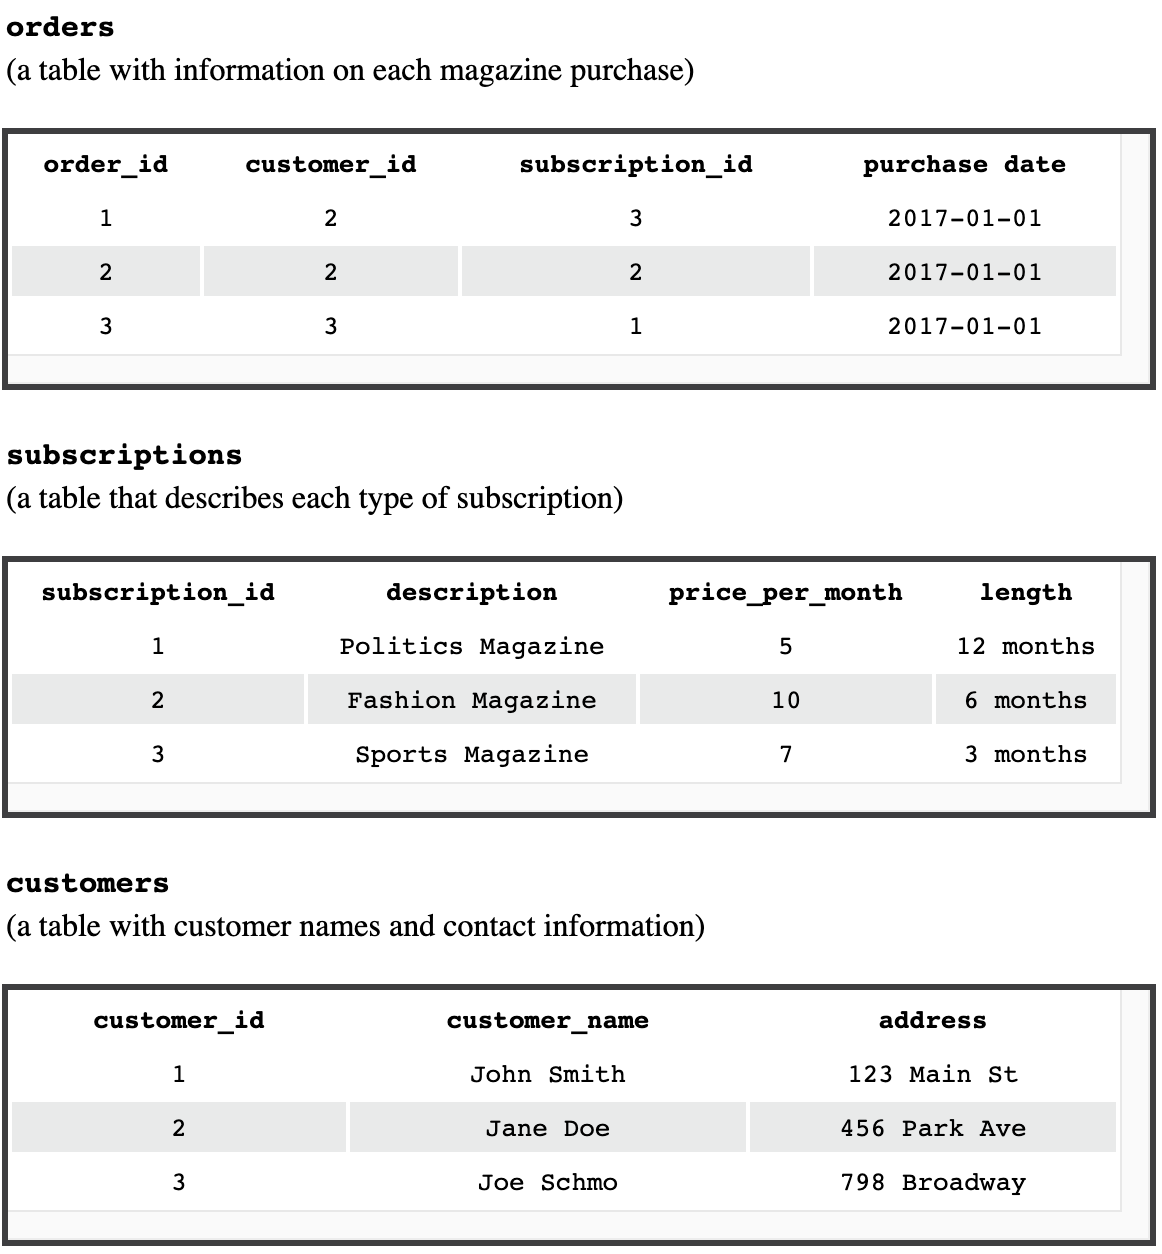
\includegraphics[scale = 0.73]{4_1}
\centering
\end{figure}
If we just look at the \colorbox{lightgray}{orders} table, we cannot really tell what has happened in each order. However, if we refer to the other tables, we can get a complete picture.

Let us examine the order with an \colorbox{lightgray}{order\_id} of 2. It was purchased by the customer with a \colorbox{lightgray}{customer\_id} of 2.

To find out the customer’s name, we look at the \colorbox{lightgray}{customers} table and look for the item with a \colorbox{lightgray}{customer\_id} value of 2. We can see that Customer 2’s name is ‘Jane Doe’ and that she lives at ‘456 Park Ave’.

Doing this kind of matching is called \textbf{joining} two tables.

\subsection{Combining Tables with SQL}
Combining tables manually is time-consuming. Luckily, SQL gives us an easy sequence for this: it is called a \colorbox{lightgray}{JOIN}.

If we want to combine orders and customers, we would type:
\begin{lstlisting}
SELECT *
FROM orders
JOIN customers
  ON orders.customer_id = customers.customer_id;
\end{lstlisting}
Let us break down this command:
\begin{enumerate}[leftmargin = *]
\item The first line selects all columns from our combined table. If we only want to select certain columns, we can specify which ones we want.
\item The second line specifies the first table that we want to look in, \colorbox{lightgray}{orders}
\item The third line uses \colorbox{lightgray}{JOIN} to say that we want to combine information from \colorbox{lightgray}{orders} with \colorbox{lightgray}{customers}.
\item The fourth line tells us how to combine the two tables. We want to match \colorbox{lightgray}{orders} table’s \colorbox{lightgray}{customer\_id} column with \colorbox{lightgray}{customers} table’s \colorbox{lightgray}{customer\_id} column.
\end{enumerate}
Because column names are often repeated across multiple tables, we use the syntax \colorbox{lightgray}{table\_name.column\_name} to be sure that our requests for columns are unambiguous. In our example, we use this syntax in the \colorbox{lightgray}{ON} statement, but we will also use it in the \colorbox{lightgray}{SELECT} or any other statement where we refer to column names.

For example: Instead of selecting all the columns using \colorbox{lightgray}{*}, if we only wanted to select \colorbox{lightgray}{orders} table’s \colorbox{lightgray}{order\_id} column and \colorbox{lightgray}{customers} table’s \colorbox{lightgray}{customer\_name} column, we could use the following query:
\begin{lstlisting}
SELECT orders.order_id,
   customers.customer_name
FROM orders
JOIN customers
  ON orders.customer_id = customers.customer_id;
\end{lstlisting}

\subsection{Inner Joins}
Let us revisit how we joined \colorbox{lightgray}{orders} and \colorbox{lightgray}{customers}. For every possible value of \colorbox{lightgray}{customer\_id} in \colorbox{lightgray}{orders}, there was a corresponding row of customers with the same \colorbox{lightgray}{customer\_id}.

But there are cases that it is not true. For instance, imagine that our \colorbox{lightgray}{customers} table was out of date, and was missing any information on customer 11. If that customer had an \colorbox{lightgray}{order} in orders, then when we perform a simple \colorbox{lightgray}{JOIN} (often called an \textit{inner join}) our result only includes rows that match our \colorbox{lightgray}{ON} condition.

\subsection{Left Joins}
If we want to combine two tables and keep some of the un-matched rows, we can do this through a command called \colorbox{lightgray}{LEFT JOIN} (or \colorbox{lightgray}{RIGHT JOIN}). A \textit{left join} will keep all rows from the first table, regardless of whether there is a matching row in the second table. The final result will keep all rows of the first table but will omit the un-matched row from the second table.

Consider the following code 
\begin{lstlisting}
SELECT *
FROM table1
LEFT JOIN table2
  ON table1.c2 = table2.c2;
\end{lstlisting}
\begin{itemize}[leftmargin = *]
\item The first line selects all columns from both tables.
\item The second line selects \colorbox{lightgray}{table1} (the “left” table).
\item The third line performs a \colorbox{lightgray}{LEFT JOIN} on \colorbox{lightgray}{table2} (the “right” table).
\item The fourth line tells SQL how to perform the join (by looking for matching values in column \colorbox{lightgray}{c2}).
\end{itemize}

\subsection{Primary Key vs Foreign Key}
Let us return to our example of the magazine subscriptions. Recall that we had three tables: \colorbox{lightgray}{orders}, \colorbox{lightgray}{subscriptions}, and \colorbox{lightgray}{customers}.

Each of these tables has a column that uniquely identifies each row of that table:
\begin{itemize}[leftmargin = *]
\item \colorbox{lightgray}{order\_id} for orders
\item \colorbox{lightgray}{subscription\_id} for subscriptions
\item \colorbox{lightgray}{customer\_id} for customers
\end{itemize}
These special columns are called \textbf{primary keys}.

Primary keys have a few requirements:
\begin{itemize}[leftmargin = *]
\item None of the values can be \colorbox{lightgray}{NULL}.
\item Each value must be unique (i.e., you cannot have two customers with the same \colorbox{lightgray}{customer\_id} in the \colorbox{lightgray}{customers} table).
\item A table can not have more than one primary key column.
\end{itemize}
Let us reexamine the \colorbox{lightgray}{orders} table:

{\rowcolors{1}{white}{yellow}
\begin{tabular}{ | m{10em} | m{10em} | m{10em} | m{10em} |}
\hline
\textbf{order\_id} & \textbf{customer\_id} & \textbf{subscription\_id} & \textbf{purchase\_date} \\
\hline
1 & 2 & 3 &  2017-01-01\\
\hline
2 & 2 & 2 &  2017-01-01\\
\hline 
3 & 3 & 1 &  2017-01-01\\
\hline 
\end{tabular}

Note that \colorbox{lightgray}{customer\_id} (the primary key for \colorbox{lightgray}{customers}) and \colorbox{lightgray}{subscription\_id} (the primary key for \colorbox{lightgray}{subscriptions}) both appear in this.

When the primary key for one table appears in a different table, it is called a \textbf{foreign key}.

So \colorbox{lightgray}{customer\_id} is a primary key when it appears in \colorbox{lightgray}{customers}, but a foreign key when it appears in \colorbox{lightgray}{orders}.

In this example, our primary keys all had somewhat descriptive names. Generally, the primary key will just be called \colorbox{lightgray}{id}. Foreign keys will have more descriptive names.

This is important because the most common types of joins will be joining a foreign key from one table with the primary key from another table. For instance, when we join \colorbox{lightgray}{orders} and \colorbox{lightgray}{customers}, we join on \colorbox{lightgray}{customer\_id}, which is a foreign key in \colorbox{lightgray}{orders} and the primary key in \colorbox{lightgray}{customers}.

\subsection{Cross Join}
So far, we have focused on matching rows that have some information in common.

Sometimes, we just want to combine all rows of one table with all rows of another table. For instance, if we had a table of shirts and a table of pants, we might want to know all the possible combinations to create different outfits. Our code might look like this:
\begin{lstlisting}
SELECT shirts.shirt_color,
   pants.pants_color
FROM shirts
CROSS JOIN pants;
\end{lstlisting}
\begin{itemize}[leftmargin = *]
\item The first two lines select the columns \colorbox{lightgray}{shirt\_color} and \colorbox{lightgray}{pants\_color}.
\item The third line pulls data from the table \colorbox{lightgray}{shirts}.
\item The fourth line performs a \colorbox{lightgray}{CROSS JOIN} with \colorbox{lightgray}{pants}.
\end{itemize}
Notice that cross joins do not require an \colorbox{lightgray}{ON} statement because we are not joining on any columns. 

If we have 3 different shirts (white, grey, and olive) and 2 different pants (light denim and black), the results might look like this:

{\rowcolors{1}{white}{yellow}
\begin{tabular}{ | m{20em} | m{20em} |}
\hline
\textbf{shirt\_color} & \textbf{pants\_color} \\
\hline
white & light denim \\
\hline
white & black \\
\hline 
grey	& light denim\\
\hline 
grey	& black \\
\hline
olive	& light denim \\
\hline
olive	& black \\
\hline
\end{tabular}

3 shirts $\times$ 2 pants = 6 combinations

A more common usage of \colorbox{lightgray}{CROSS JOIN} is when we need to compare each row of a table to a list of values.

Let us return to our \colorbox{lightgray}{newspaper} subscriptions. This table contains two columns that we have not discussed yet:
\begin{itemize}[leftmargin = *]
\item \colorbox{lightgray}{start\_month}: the first month where the customer subscribed to the print newspaper (i.e., \colorbox{lightgray}{2} for February)
\item \colorbox{lightgray}{end\_month}: the final month where the customer subscribed to the print newspaper
\end{itemize}
Suppose we wanted to know how many users were subscribed during each month of the year. For each month (\colorbox{lightgray}{1}, \colorbox{lightgray}{2}, \colorbox{lightgray}{3}) we would need to know if a user was subscribed. 
\begin{lstlisting}
SELECT month, COUNT(*)
FROM newspaper 
CROSS JOIN months 
WHERE start_month <= month AND end_month >= month 
GROUP BY month; 
\end{lstlisting}

\subsection{Union}
Sometimes we just want to stack one dataset on top of the other. The \colorbox{lightgray}{UNION} operator allows us to do that.

Suppose we have two tables and they have the same columns.

\colorbox{lightgray}{table1}:

{\rowcolors{1}{white}{yellow}
\begin{tabular}{ | m{20em} | m{20em} |}
\hline
\textbf{pokemon} & \textbf{type} \\
\hline
Bulbasaur & Grass \\
\hline
Charmander & Fire\\
\hline 
Squirtle & Water\\
\hline
\end{tabular}

\colorbox{lightgray}{table2}:

{\rowcolors{1}{white}{yellow}
\begin{tabular}{ | m{20em} | m{20em} |}
\hline
\textbf{pokemon} & \textbf{type} \\ 
\hline
Snorlax & Normal \\
\hline
\end{tabular}

If we combine these two with \colorbox{lightgray}{UNION}:
\begin{lstlisting}
SELECT *
FROM table1
UNION
SELECT *
FROM table2;
\end{lstlisting}
The result would be:

{\rowcolors{1}{white}{yellow}
\begin{tabular}{ | m{20em} | m{20em} |}
\hline
\textbf{pokemon} & \textbf{type} \\ 
\hline
Bulbasaur & Grass \\ 
\hline
Charmander & Fire \\
\hline
Squirtle & Water \\ 
\hline
Snorlax & Normal \\
\hline
\end{tabular}

SQL has strict rules for appending data:
\begin{itemize}[leftmargin = *]
\item Tables must have the same number of columns.
\item The columns must have the same data types in the same order as the first table.
\end{itemize}

\subsection{With}
Often times, we want to combine two tables, but one of the tables is the result of another calculation.

Let us return to our magazine order example. Our marketing department might want to know a bit more about our customers. For instance, they might want to know how many magazines each customer subscribes to. We can easily calculate this using our \colorbox{lightgray}{orders} table:
\begin{lstlisting}
SELECT customer_id,
   COUNT(subscription_id) AS "subscriptions"
FROM orders
GROUP BY customer_id;
\end{lstlisting}
This query is good, but a \colorbox{lightgray}{customer\_id} is not terribly useful for our marketing department, they probably want to know the customer's name.

We want to be able to join the results of this query with our \colorbox{lightgray}{customers} table, which will tell us the name of each customer. We can do this by using a \colorbox{lightgray}{WITH} clause.
\begin{lstlisting}
WITH previous_results AS (
   SELECT ...
   ...
   ...
   ...
)
SELECT *
FROM previous_results
JOIN customers
  ON _____ = _____;
\end{lstlisting}
\begin{itemize}[leftmargin = *]
\item The \colorbox{lightgray}{WITH} statement allows us to perform a separate query (such as aggregating customer’s subscriptions)
\item \colorbox{lightgray}{previous\_results} is the alias that we will use to reference any columns from the query inside of the \colorbox{lightgray}{WITH} clause
\item We can then go on to do whatever we want with this temporary table (such as join the temporary table with another table)
\end{itemize}
Essentially, we are putting a whole first query inside the parentheses \colorbox{lightgray}{()} and giving it a name. After that, we can use this name as if it is a table and write a new query using the first query.

\subsection{Review}
We learned about relationships between tables in relational databases and how to query information from multiple tables using SQL.
\begin{itemize}
\item \colorbox{lightgray}{JOIN} will combine rows from different tables if the join condition is true.
\item \colorbox{lightgray}{LEFT JOIN} will return every row in the left table, and if the join condition is not met, NULL values are used to fill in the columns from the right table.
\item \colorbox{lightgray}{Primary key} is a column that serves a unique identifier for the rows in the table.
\item \colorbox{lightgray}{Foreign key} is a column that contains the primary key to another table.
\item \colorbox{lightgray}{CROSS JOIN} lets us combine all rows of one table with all rows of another table.
\item \colorbox{lightgray}{UNION} stacks one dataset on top of another.
\item \colorbox{lightgray}{WITH} allows us to define one or more temporary tables that can be used in the final query.
\end{itemize}

\newpage
\section{Analytic Functions}
\subsection{Introduction}
Now we will learn how to define \textit{analytic functions}, which also operate on a set of rows like \textit{aggregate functions}. However, unlike aggregate functions, analytic functions return a (potentially different) value for each row in the original table.

Analytic functions allow us to perform complex calculations with relatively straightforward syntax. For instance, we can quickly calculate moving averages and running totals, among other quantities.

\subsection{Syntax}
To understand how to write analytic functions, we will work with a small table containing data from two different people who are training for a race. The \colorbox{lightgray}{id} column identifies each runner, the \colorbox{lightgray}{date} column holds the day of the training session, and \colorbox{lightgray}{time} shows the time (in minutes) that the runner dedicated to training. 
{\rowcolors{1}{white}{yellow}
\begin{tabular}{ | m{13em} | m{13em} | m{13em} | }
\hline
\textbf{id} & \textbf{date} & \textbf{time} \\ 
\hline
1 & 2019-07-05 & 22 \\ 
\hline
1 & 2019-04-15 & 26 \\ 
\hline
2 & 2019-02-06 & 28 \\ 
\hline
1 & 2019-01-02 & 30 \\ 
\hline
1 & 2019-08-30 & 30 \\
\hline
1 & 2019-03-09 & 22 \\
\hline  
\end{tabular}

Say we would like to calculate a \textit{moving average} of the training times for each runner, where we always take the average of the current and previous training sessions. We can do this with the following query:
\begin{lstlisting}
SELECT *, 
	AVG(time) OVER(
				   PARTITION BY id 
				   ORDER BY date 
				   ROWS BETWEEN 1 PRECEDING AND CURRENT ROW 
				   ) as avg_time 
FROM table; 
\end{lstlisting}
All analytic functions have an \colorbox{lightgray}{OVER} clause, which defines the sets of rows used in each calculation. The \colorbox{lightgray}{OVER} clause has three (optional) parts:
\begin{itemize}[leftmargin = *]
\item The \colorbox{lightgray}{PARTITION BY} clause divides the rows of the table into different groups. In the query above, we divide by \colorbox{lightgray}{id} so that the calculations are separated by runner.
\item The \colorbox{lightgray}{ORDER BY} clause defines an ordering within each partition. In the sample query, ordering by the date column ensures that earlier training sessions appear first.
\item The final clause (\colorbox{lightgray}{ROWS BETWEEN 1 PRECEDING AND CURRENT ROW}) is known as a \textbf{window frame} clause. It identifies the set of rows used in each calculation. We can refer to this group of rows as a \textbf{window}. (Actually, analytic functions are sometimes referred to as \textbf{analytic window functions} or \textbf{window functions}.)
\end{itemize}
\begin{figure}[H]
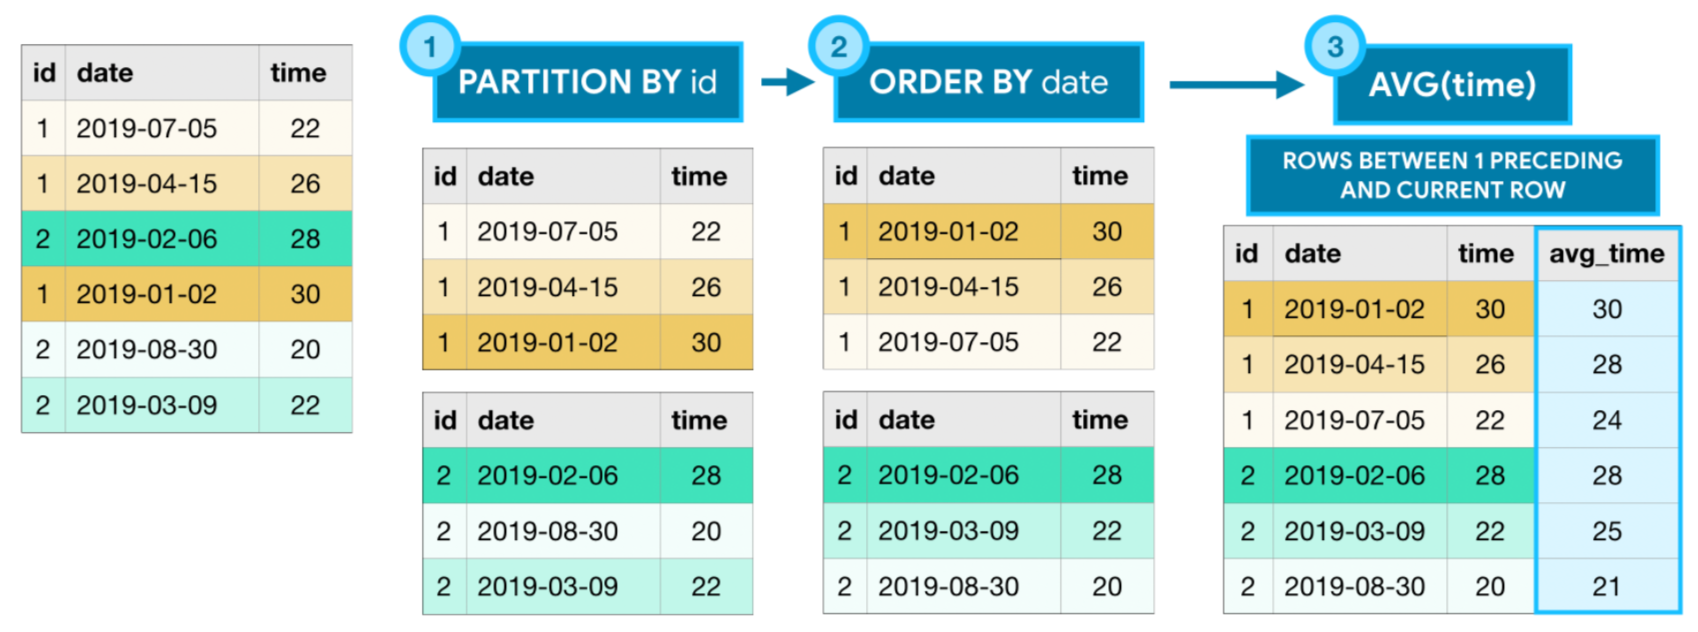
\includegraphics[scale = 0.6]{5_1}
\centering
\end{figure}

\subsection{(More on) window frame clauses}
There are many ways to write window frame clauses:
\begin{itemize}[leftmargin = *]
\item \colorbox{lightgray}{ROWS BETWEEN 1 PRECEDING AND CURRENT ROW} - the previous row and the current row.
\item \colorbox{lightgray}{ROWS BETWEEN 3 PRECEDING AND 1 FOLLOWING} - the 3 previous rows, the current row, and the following row.
\item \colorbox{lightgray}{ROWS BETWEEN UNBOUNDED PRECEDING AND UNBOUNDED FOLLOWING} - all rows in the partition.
\end{itemize}
Of course, this is not an exhaustive list, and you can imagine that there are many more options. In the code below, you will see some of these clauses in action.

\subsection{Three types of analytic functions}
The example above uses only one of many analytic functions. BigQuery supports a wide variety of analytic functions, and we will explore a few here. For a complete listing, you can take a look at the \href{https://cloud.google.com/bigquery/docs/reference/standard-sql/analytic-function-concepts}{documentation}.
\begin{enumerate}[leftmargin = *]
\item Analytic aggregate functions
As you might recall, \colorbox{lightgray}{AVG()} (from the example above) is an aggregate function. The \colorbox{lightgray}{OVER} clause is what ensures that it is treated as an analytic (aggregate) function. \textbf{Aggregate functions} take all of the values within the window as input and return a single value.
\begin{itemize}
\item \colorbox{lightgray}{MIN()} (or \colorbox{lightgray}{MAX()}) - Returns the minimum (or maximum) of input values
\item \colorbox{lightgray}{AVG()} (or \colorbox{lightgray}{SUM()}) - Returns the average (or sum) of input values
\item \colorbox{lightgray}{COUNT()} - Returns the number of rows in the input
\end{itemize}
\item Analytic navigation functions
\textbf{Navigation functions} assign a value based on the value in a (usually) different row than the current row.
\begin{itemize}
\item \colorbox{lightgray}{FIRST\_VALUE()} (or \colorbox{lightgray}{LAST\_VALUE()}) - Returns the first (or last) value in the input
\item \colorbox{lightgray}{LEAD()} (and \colorbox{lightgray}{LAG()}) - Returns the value on a subsequent (or preceding) row
\end{itemize}
\item Analytic numbering functions
\textbf{Numbering functions} assign integer values to each row based on the ordering.
\begin{itemize}
\item \colorbox{lightgray}{ROW\_NUMBER()} - Returns the order in which rows appear in the input (starting with 1)
\item \colorbox{lightgray}{RANK()} - All rows with the same value in the ordering column receive the same rank value, where the next row receives a rank value which increments by the number of rows with the previous rank value.
\end{itemize}
\end{enumerate}

\newpage
\section{Nested and Repeated Data}
Now we will learn how to query nested and repeated data. These are the most complex data types that you can find in BigQuery datasets. 

\subsection{Nested Data}
Consider a hypothetical dataset containing information about pets and their toys. We could organize this information in two different tables (a \colorbox{lightgray}{pets} table and a \colorbox{lightgray}{toys} table). The \colorbox{lightgray}{toys} table could contain a \colorbox{lightgray}{Pet\_ID} column that could be used to match each toy to the pet that owns it.

Another option in BigQuery is to organize all of the information in a single table, similar to the \colorbox{lightgray}{pets\_and\_toys} table below.
\begin{figure}[H]
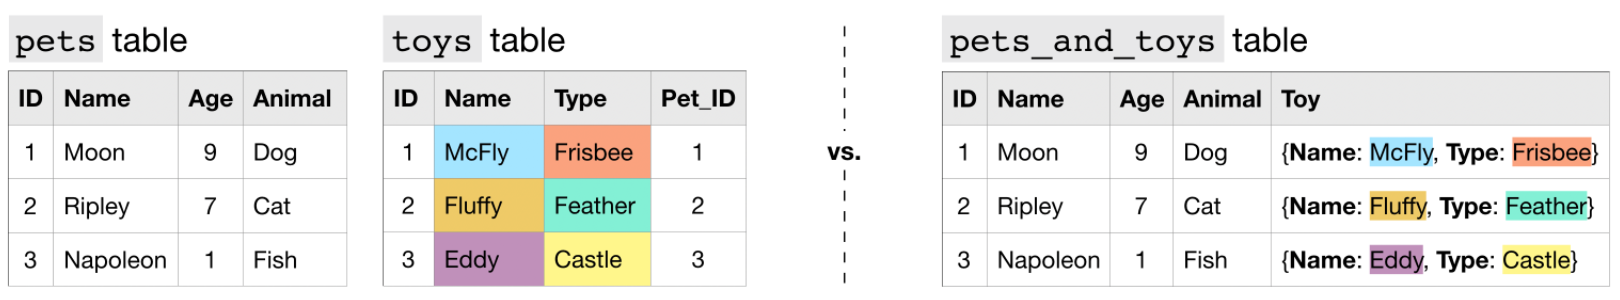
\includegraphics[scale = 0.6]{6_1}
\centering
\end{figure}
\vspace{-4mm}
In this case, all of the information from the \colorbox{lightgray}{toys} table is collapsed into a single column (the \colorbox{lightgray}{Toy} column in the \colorbox{lightgray}{pets\_and\_toys} table). We refer to the \colorbox{lightgray}{Toy} column in the \colorbox{lightgray}{pets\_and\_toys} table as a \textbf{nested column}, and say that the \colorbox{lightgray}{Name} and \colorbox{lightgray}{Type} fields are nested inside of it.

Nested columns have type \textbf{STRUCT} (or type \textbf{RECORD}). This is reflected in the table schema below.
\begin{figure}[H]
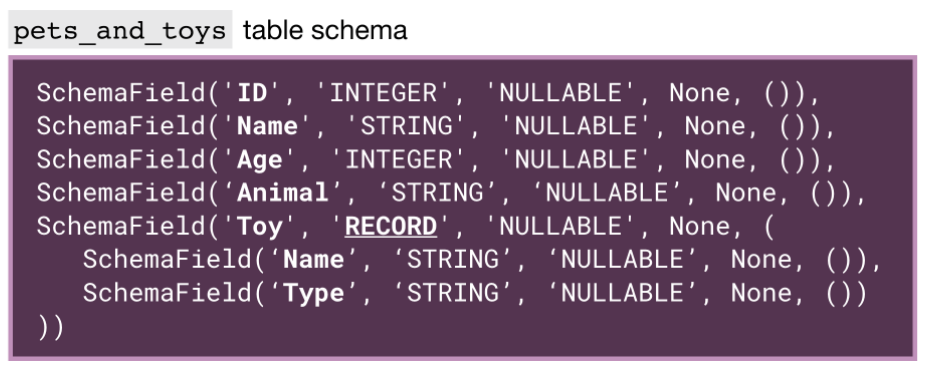
\includegraphics[scale = 0.8]{6_2}
\centering
\end{figure}
\vspace{-4mm}
To query a column with nested data, we need to identify each field in the context of the column that contains it:
\begin{itemize}[leftmargin = *]
\item \colorbox{lightgray}{Toy.Name} refers to the \colorbox{lightgray}{Name} field in the \colorbox{lightgray}{Toy} column
\item \colorbox{lightgray}{Toy.Type} refers to the \colorbox{lightgray}{Type} field in the \colorbox{lightgray}{Toy} column.
\end{itemize}
\begin{lstlisting}
SELECT Name AS Pet_Name, 
	      Toy.Name AS Toy_Name, 
	      Toy.Type AS Toy_Type
FROM pets_and_toys;
\end{lstlisting}
The code above yields: 
\begin{figure}[H]
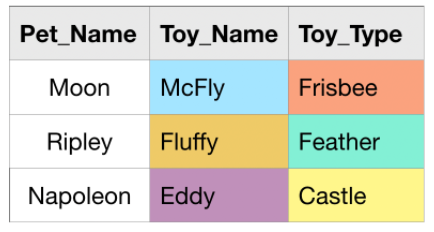
\includegraphics[scale = 0.7]{6_3}
\centering
\end{figure}
\vspace{-4mm}
Otherwise, our usual rules remain the same - we need not change anything else about our queries.

\subsection{Repeated Data}
Now consider the case where each pet can have multiple toys. In this case, to collapse this information into a single table, we need to leverage a different datatype.
\begin{figure}[H]
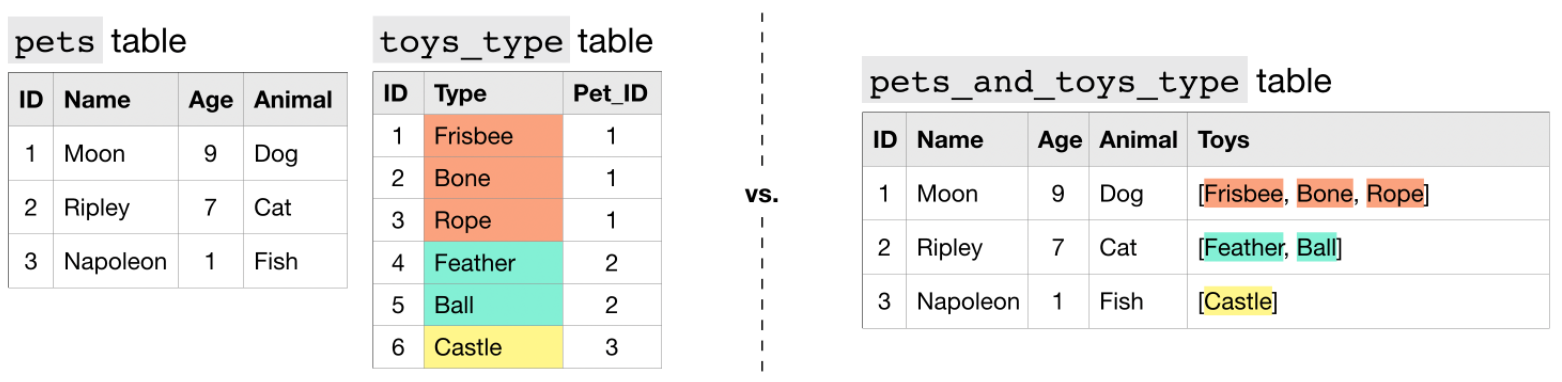
\includegraphics[scale = 0.65]{6_4}
\centering
\end{figure}
\vspace{-4mm}
We say that the \colorbox{lightgray}{Toys} column contains \textbf{repeated data}, because it permits more than one value for each row. This is reflected in the table schema below, where the mode of the \colorbox{lightgray}{Toys} column appears as \colorbox{lightgray}{REPEATED}.
\begin{figure}[H]
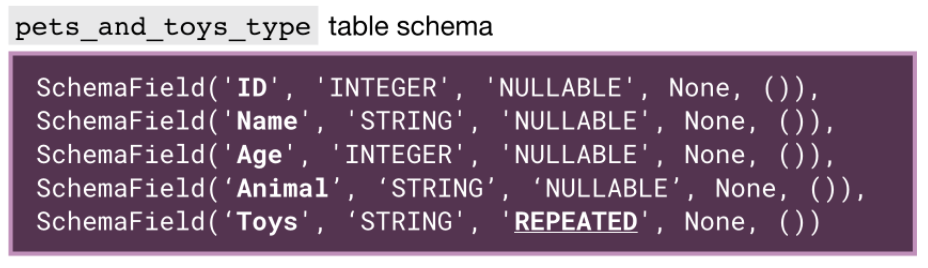
\includegraphics[scale = 0.8]{6_5}
\centering
\end{figure}
Each entry in a repeated field is an \colorbox{lightgray}{ARRAY}, or an ordered list of (zero or more) values with the same datatype. For instance, the entry in the \colorbox{lightgray}{Toys} column for \colorbox{lightgray}{Moon} the Dog is \textbf{[Frisbee, Bone, Rope]}, which is an \colorbox{lightgray}{ARRAY} with three values.

When querying repeated data, we need to put the name of the column containing the repeated data inside an \colorbox{lightgray}{UNNEST()} function.
\begin{lstlisting}
SELECT Name AS PetName,
	       Toy_Type
FROM pets_and_toys_type
	UNNEST(Toys) AS Toy_Type;
\end{lstlisting}
\begin{figure}[H]
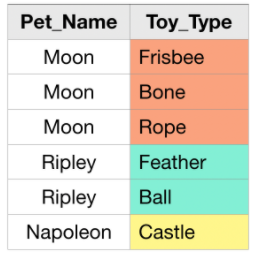
\includegraphics[scale = 0.9]{6_6}
\centering
\end{figure}
\vspace{-4mm}
This essentially flattens the repeated data (which is then appended to the right side of the table) so that we have one element on each row.

\subsection{Nested and repeated data}
If pets can have multiple toys, and we would like to keep track of both the name and type of each toy, we can make the \colorbox{lightgray}{Toys} column both \textbf{nested} and \textbf{repeated}.
\begin{figure}[H]
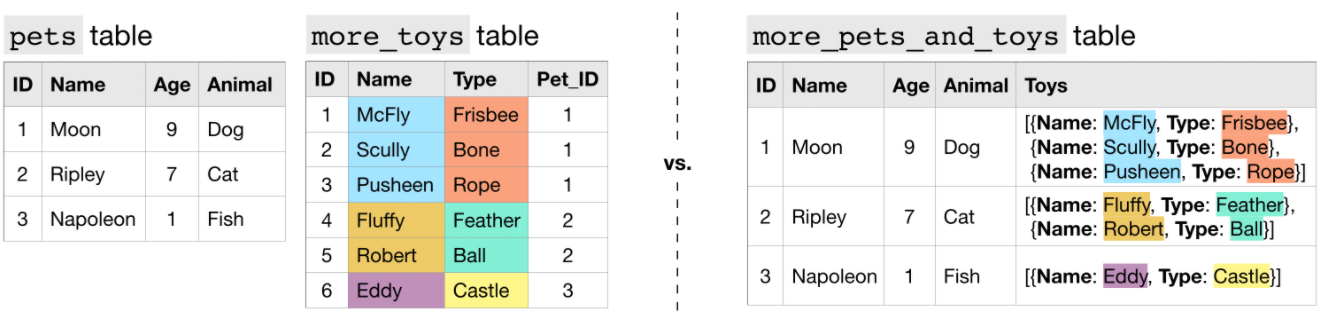
\includegraphics[scale = 0.75]{6_7}
\centering
\end{figure}
\vspace{-4mm}
In the \colorbox{lightgray}{more\_pets\_and\_toys} table above, \colorbox{lightgray}{Name} and \colorbox{lightgray}{Type} are both fields contained within the \colorbox{lightgray}{Toys} \colorbox{lightgray}{STRUCT}, and each entry in both \colorbox{lightgray}{Toys.Name} and \colorbox{lightgray}{Toys.Type} is an \colorbox{lightgray}{ARRAY}.
\begin{figure}[H]
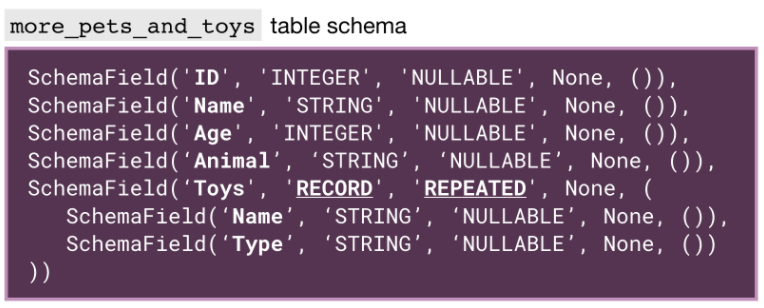
\includegraphics[scale = 0.9]{6_8}
\centering
\end{figure}
\vspace{-4mm}
Let us look at a sample query. 
\begin{lstlisting}
SELECT Name AS Pet_Name, 
	      t.Name AS Toy_Name, 
	      t.Type AS Toy_Type
FROM more_pets_and_toys 
	UNNEST(Toys) AS t; 
\end{lstlisting}
The code above generates:

\begin{figure}[H]
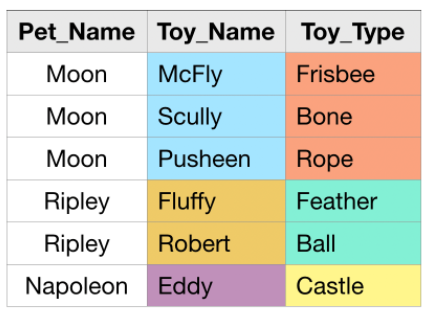
\includegraphics[scale = 0.8]{6_9}
\centering
\end{figure}
\vspace{-4mm}

Since the \colorbox{lightgray}{Toys} column is repeated, we flatten it with the \colorbox{lightgray}{UNNEST()} function. And, since we give the flattened column an alias of \colorbox{lightgray}{t}, we can refer to the \colorbox{lightgray}{Name} and \colorbox{lightgray}{Type} fields in the \colorbox{lightgray}{Toys} column as \colorbox{lightgray}{t.Name} and \colorbox{lightgray}{t.Type}, respectively.

\end{document}
